%# -*- coding: utf-8-unix -*-
% !TEX program = xelatex
% !TEX root = ../thesis.tex
% !TEX encoding = UTF-8 Unicode
%%==================================================
%% chapter02.tex for SJTU Master Thesis
%% based on CASthesis
%% modified by wei.jianwen@gmail.com
%% Encoding: UTF-8
%%==================================================

\chapter{基于深度强化学习的NL2SQL生成}
\label{chap:enl2sql}

\section{研究问题}

随着计算机技术的快速发展与应用,关系型数据库被广泛应用于教育、医疗、商业等领域。
作为信息存储的载体,越来越多的软件开发和业务人员正频繁使用SQL查询语句来读取关系型数据库中的数据。
SQL语句用法多样且功能强大,但对于一个没有技术背景的使用者来说却是一场噩梦。
即便是一名专业的软件人员,在面对数据库中众多的实体以及每个实体都有自己独特的含义时,想要把SQL语句写正确也不是一件容易的事情。
因此,学术界和工业界一直都在思考如何更快更好地使用SQL语句来读取数据,其中最理想和最直接的方式便是直接让使用者使用自然语言从数据库中获取所需信息。

实现这个目标的关键在于如何去理解自然语言语句的意图并讲其映射到SQL语句上,简称为NL2SQL(Nature Language To SQL Statement),即自然语言生成SQL查询语句任务。
在NL2SQL任务中,一个典型的例子如图\ref{fig:nl2sqlexample}给出。

\begin{figure}[!htp]
    \centering
    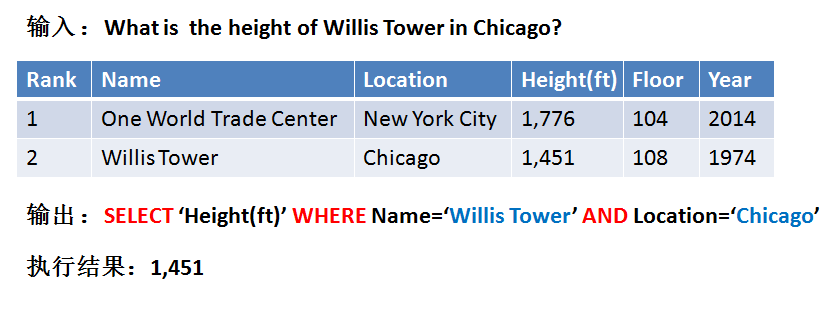
\includegraphics[width=15cm]{example/nl2sql.png}
    \bicaption[这里将出现在插图索引中]
      {NL2SQL的一个典型示例}
      {English caption}
    \label{fig:nl2sqlexample}
  \end{figure}

图\ref{fig:nl2sqlexample}为WikiSQL数据集[!!引用!!]中的一个样例。
WikiSQL数据集是纯自然语言生成SQL查询语句的第一个数据集。
其中包含80654组自然语言问句及其对应的SQL查询语句,涵盖24241张从Wikipedia中获取的数据表。
从图中可以看到,NL2SQL任务的输入实际包括两部分:自然语言问题以及一个简单的数据表schema(schema代表数据表及表中的列)。

WikiSQL数据集中SQL查询语句具有一定的约束条件,必须符合如下模板:

\begin{table}[!hpb]
    \centering
    \bicaption[指向一个表格的表目录索引]
      {SQL查询语句模板}
      {A Table}
    \label{nli:sqlmb}
    \begin{tabular}{@{}llr@{}} \toprule
      % \multicolumn{2}{c}{Item} \\ \cmidrule(r){1-2}
    %   节点类型 & 对应的SQL组件\\\midrule
    \emph{SELECT   agg   selcol   WHERE   col   op   val   (AND   col   op   val)*}\\\bottomrule
  
      % Animal & Description & Price (\$)\\ \midrule
      % Gnat & per gram & 13.65 \\
      % & each & 0.01 \\
      % Gnu & stuffed & 92.50 \\
      % Emu & stuffed & 33.33 \\
      % Armadillo & frozen & 8.99 \\ \bottomrule
    \end{tabular}
  \end{table}

  在\ref{nli:sqlmb}中,\emph{selcol}代表表中的列名,\emph{agg}代表聚合操作(例如:COUNT,SUM或空),
  \emph{WHERE}后面为由一系列过滤调教构成的子句,每个\emph{op}代表一个过滤操作(例如:“=”),\emph{val}代表出现在自然语言问句中的过滤值。
  值得注意的是,尽管模板中的过滤条件服从标准的线性顺序,但由于存在\emph{AND}符号,所以过滤条件的先后顺序是无关紧要的。

  在后文中,我们声明如下一些表示:总输入表示为$x$,其包含由单词$w_{i}$组成的自然语言问题$w$以及由列名$c_{j}$组成的单张表的schema $c$(其中,列名$c_{j}$可由单个或多个单词组成)。
  最后,我们的模型需要生成一条可执行的SQL查询语句$y$作为输出。

\section{相关技术}
\subsection{NL2SQL研究现状}
\subsection{深度学习}
\subsection{强化学习}
\subsection{语义解析}
\section{解决方案}

\subsection{增强解析器模型}
\label{enl2sql:zqjxqmx}
针对每个输入$x$来生成结构化的输出$y$的过程可以被分解成为一系列的语义解析决策的过程。
所以,增强解析器模型的基本思路为:解析器从初始状态启动并不断根据学习的策略采取不同的操作。
每个动作(action)都会将解析器从一个状态(state)转移为另一个状态,知道解析器到达它的最终状态并停止。
在解析器的最终状态下,我们可以获取一个完整的输出$y$。
我们采取一种概率的方法来对整个的策略(policy)建模。
它可以对由输入$x$产生的有效的动作(action)的集合以及解码器产生的历史行为进行概率分布进行预测。
所以,整个增量语义解析器的训练目标就转换为了如何优化一个参数化的策略的问题。

% , 其中$\theta$为模型参数。
\begin{equation}
    \label{enl2sql:eq1}
    % Sim \left ( n ,\right v) = \max\left ( Sim_{wup}\left ( n ,\right v) ,\right Sim_{gram}\left ( n ,\right v))
    % Sim(n,v) = \max(Sim_{wup}(n,v),Sim_{gram}(n,v))
    % P_{\theta}(y|x) = P_{\theta}(\boldsymbol{a}|x),   \theta为模型参数
    P_{\theta}(y|x) = P_{\theta}(\boldsymbol{a}|x),  \qquad \theta\text{为模型参数}
\end{equation}

根据公式\ref{enl2sql:eq1},通过执行动作(action)序列$\boldsymbol{a} = \{a_{1},a_{2},...,a_{k}\}$,解析器将被不断引导并从初始状态转换为包含输出$y$的最终状态。
在此,我们需要假设每个输出$y$有且仅有一个对应的动作序列$\boldsymbol{a}$(详见\ref{enl2sql:ndo}节内容)。
行动序列的概率$P_{\theta}(\boldsymbol{a}|x)$可展开为增量策略概率的乘积(公式\ref{enl2sql:eq2}):

\begin{equation}
    \label{enl2sql:eq2}
    % Sim \left ( n ,\right v) = \max\left ( Sim_{wup}\left ( n ,\right v) ,\right Sim_{gram}\left ( n ,\right v))
    % Sim(n,v) = \max(Sim_{wup}(n,v),Sim_{gram}(n,v))
    P_{\theta}(\boldsymbol{a}|x) = \prod^k_{i=1}P_{\theta}(a_{i}|x,a_{<i}),   \qquad |\boldsymbol{a}| = k
\end{equation}

在推断(inference)期间,我们的模型并非尝试枚举整个输出空间并找到最高的得分$\boldsymbol{a}^{*} = \mathop{\arg\max}_{\boldsymbol{a}} P_{\theta}(\boldsymbol{a}|x)$,
而是在解码器中采用了一种贪心的方法:在每一步都根据策略(policy)来选择得分最高的行动,即$a^{*}_{i} = \mathop{\arg\max}_{a_{i}} P_{\theta}(a_{i}|x,a^{*}_{<i})$。

在后面的几节中,我们将给出解析器状态(state)的定义以及动作(action)清单,还会详细介绍整个基于编码器-解码器神经网络体系结构的增强解析器模型。

% \begin{figure}[!htp]
%   \centering
%   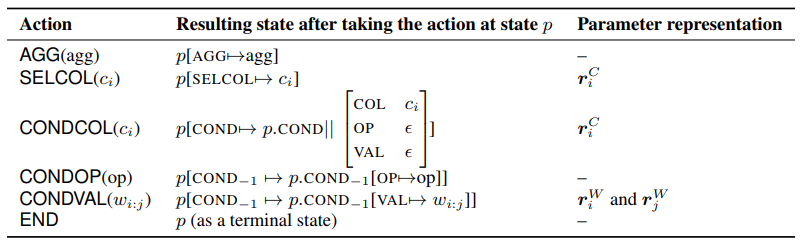
\includegraphics[width=20cm]{example/incsql.png}
%   \bicaption[这里将出现在插图索引中]
%     {中文题图}
%     {English caption}
%   \label{fig:SRR}
% \end{figure}

\subsection{动作序列}
\label{enl2sql:dzxl}

首先,我们给出对应于图\ref{fig:nl2sqlexample}中示例的完全解析之后的结构化表示:
% $\begin{Bmatrix}
%   1 & 2 \\
%   4 & 3 \\
% \end{Bmatrix}$
% \begin{bmatrix}
  
% \end{bmatrix}

$\begin{bmatrix}
  AGG    &  NONE  \\
  SELCOL &  Height(ft) \\
  COND   &   \langle
  % \begin{Bmatrix}
    \begin{bmatrix}
      COL  &  Name \\
      OP   &  =    \\
      VAL  &  “Willis Tower”\\
    \end{bmatrix}
    ,
    \begin{bmatrix}
      COL  &  Location \\
      OP   &  =    \\
      VAL  &  “Chicago”\\
    \end{bmatrix}
    % \end{Bmatrix}
    \rangle
  \end{bmatrix}$

因此,解析器的中间状态就被这样分部表示,其中一些尚未填充的特征值表示为$\epsilon$。
解析器的初始状态$p_{0}$的值为空和空列表,表示为$\begin{bmatrix}
  AGG    &  \epsilon  \\
  SELCOL &  \epsilon \\
  COND   &   \langle \rangle\\
  \end{bmatrix}$。

除此之外,我们还需要定义动作(action)清单。每个动作可以将解析器的状态从一个状态转换为另一个状态,即 $p \rightarrow p_{'}$ 。
我们设$p = \begin{bmatrix}
  AGG    &  agg  \\
  SELCOL &  selcol \\
  COND   &   cond\\
  \end{bmatrix}$,并且在表\ref{enl2sql:dzqd}中给出每个动作执行后的转移状态$p'$。

  \begin{table}[!hpb]
    \centering
    \bicaption[指向一个表格的表目录索引]
      {动作(action)清单}
      {A Table}
    \label{enl2sql:dzqd}
    \begin{tabular}{@{}llr@{}} \toprule
      % \multicolumn{2}{c}{Item} \\ \cmidrule(r){1-2}
      \textbf{动作(action)} & \textbf{由状态}$p$\textbf{执行该动作之后的状态} & \textbf{参数表示}\\\midrule
      % 1  & 	Q -> ( SClause ) ( ComplexCondition ) *\\
      AGG($agg$)  &  $p[AGG \mapsto agg]$  & - \\
      SELCOL($c_i$)  &  $p[SELCOL \mapsto c_i]$  & $r^C_i$ \\
      CONDCOL($c_i$)  &  $p[COND \mapsto p.COND||\begin{bmatrix}
        COL    &  c_i  \\
        OP &  \epsilon \\
        VAL   &   \epsilon\\
        \end{bmatrix}]$  &  $r^C_i$\\
      CONDOP(op)  &  $p[COND_{-1} \mapsto p.COND_{-1}[OP \mapsto op]]$  & -\\
      CONDVAL($w_{i:j}$)  &  $p[COND_{-1} \mapsto p.COND_{-1}[VAL \mapsto w_{i:j}]]$  &  $r^W_i and r^W_j$\\
      END  &  $p$(最终状态)  &  -\\\bottomrule
    \end{tabular}
  \end{table}

需要说明的是,在表\ref{enl2sql:dzqd}中,在解码器中所使用的参数表示将在\ref{enl2sql:decoder}节中进行解释;
$p[AGG \mapsto agg]$表示与状态$p$处于同一状态,不过其特征值$AGG$已经被赋值为$agg$;
$||$表示列表展开;$COND_{-1}$表示在列表中的上一个元素;


值得注意的是,动作$CONDVAL$会从输入问句$w$中选择所需的文字段$w_{i:j}$。
但这样做会导致一个问题,它将产生大量的动作,其数量级为问题长度的二次方。
因此,我们将动作$CONDVAL$分解为两个连续的子动作,一个去选择起始位置$w_i$,另一个则选择终止位置$w_j$。
在动作序列的最后,我们需要增加一个$END$动作来执行解析过程并使解析器进入结束状态。
举例来说,图\ref{fig:nl2sqlexample}中的例子可以看作是如下的一个动作序列:
\begin{enumerate}
  \item $AGG(NONE)$
  \item $SELCOL(c_3)$
  \item $CONDCOL(c_1)$
  \item $CONDOP(=)$
  \item $CONDVAL(w_{5:6})$
  \item $CONDCOL(c_2)$
  \item $CONDOP(=)$
  \item $CONDVAL(w_{8:8})$
\end{enumerate}
% ${AGG(NONE),SELCOL(c_3),CONDCOL(c_1),CONDOP(=),CONDVAL(w_{5:6}),CONDCOL(c_2),CONDOP(=),CONDVAL(w_{8:8})}$

该节中的定义是基于所有有效序列都具有AGG  SELCOL  (CONDCOL  CONDOP  CONDVAL)* END形式的假设之上。
也就保证了我们可以从所有的最终状态中提取出完整的逻辑形式出来。
对于其他不同结构的SQL语句来说,我们还需要重新设计动作的清单以及解析器的状态。


\subsection{编码器}
\label{enl2sql:encoder}

增强解析器模型的架构如图xx所示。

增强解析器模型包含编码器和解码器两个部分,其中编码器的具体步骤如下:
\begin{enumerate}
  \item 对于输入的句子$w$中的每个单词$w_i$,先将其使用词向量进行向量编码(word embedding[!!引用!!])。
  \item 将其送入一个双向的长短期记忆网络(bi-directional Long Short-Term Memory,简称bi-LSTM),其中每个细胞(cell)会有一个隐状态$h^W_i$。
  \item 由于一个列名可能由一个或多个单词构成,我们对每个列名先进行词向量编码并输入一个bi-LSTM中,再使用从bi-LSTM中得到的最终的隐状态作为列名初始表示(initial representation)。
  \item 使用自注意力机制(self-attention[!!引用!!])将该初始表示转换为$h^C_j$。
  \item 在得到基于内容的表示$h^W_i$和$h^C_j$之后,使用cross-serial dot-product attention[!!引用!!]得到$h^C_j$和$h^W_i$的加权平均值并作为单词$w_i$和$c_j$的上下文向量。
  \item 将这两个上下文向量进行拼接并分别送入使用自然语言问题和列名作为输入的bi-LSTM中。这两个LSTM网络的隐状态就是我们所期望的和上下文相关的表达$r^W_i$和$r^C_j$。
\end{enumerate}


\subsection{解码器}
\label{enl2sql:decoder}

在\ref{enl2sql:encoder}节中,我们已经获得了对于单词$w_i$上下文相关的表示$r^W_i$和以及列名$c_j$的上下文相关的表示$r^C_j$。
接下来是解码器部分的设计与细节。

首先,解码器的目标是为了对由输入$x$和历史活动$a_{<i}$构成的概率分布$P_{\theta}(a|x,a_{<i})$进行建模。其主要包括以下两点挑战:
\begin{enumerate}
  \item 活动(action)的不确定性:所有活动均需要取决于输入以及当前解析器的状态,不存在固定的活动。
  \item 解析器的决策完全依赖于上下文信息:解析器依赖于解码历史信息以及输入的问题和列名信息。
\end{enumerate}

为了解决第一个问题,我们使用了基于LSTM的解码器架构并使用活动的独立打分机制。
模型给每个候选的活动$a$打上分数$s_a$并且使用$softmax$函数将分数正则化(normalize)到一个概率分布上。
对于时刻$i$来说,我们用$h^{DEC}_i$来表示当前解码器的隐状态并且使用双线性函数$s_a = (h^{DEC}_i)^T U^A r^A_a$来给分数$a$建模。
双线性函数中$r^A_i$就是活动$a$的向量表示并且是由活动嵌入(action embedding)和参数表示(parameter representation)建模得到,
其中参数表示已经在表\ref{enl2sql:dzqd}中给出。

我们使用dot-product attention mechanism[!!引用!!]来捕获解析器的决策和输入的问题以及列名之间的依赖关系。
之后,将前一时刻$i$的输出活动表示$r^A_{a_i}$、自然语言问句的注意力向量$e^W_i$以及列名的注意力向量$e^C_i$拼接在一起,
作为$i+1$时刻的LSTM解码器的第一层的输入。
其中,向量$e^C_i = \sum_j \alpha_{i,j} r^C_j$,  $\alpha \propto h^{DEC}_i \cdot r^C_j$。
向量$e^W_i$的定义相似可得。



\subsection{解决的一些问题}
\label{enl2sql:ndo}

在前文中,我们做出过一个假设,即每个自然语言问题都只会对应一条SQL查询语句,并且每个查询语句都只会对应一个正确的动作序列。
实际上,这个假设并不能完全成立。
一个简单的例子就是出现在WHERE子句里面的过滤条件的顺序并不确定,不同的过滤条件的顺序将会导致不同的动作序列。
除此之外,我们在\ref{enl2sql:icn}节中还介绍了另一个会产生歧义的情况,它会产生一个自然语言问题可以转换为多种SQL查询语句且其执行结果仍保持一致的问题。
对于最终用户而言,这些查询语句其实是完全等效的。

针对上述的两种情况,本文会将每个训练样本转换为多个序列以供参考并且在训练过程中使用多种目标策略。
得益于语法分析领域的灵感,本文会采用一个非确定的预言(oracle)从而使得解析器可以在多个动作序列中进行探索。
特别注意的是,在前文中所述的训练机制都是采用基于静态预言而非非确定预言的。

我们假定预言(oracle)$O$可在时刻$t$返回一组正确且连续的动作$O(x,a_{<t})$。
其中,将$O(x,a_{<t})$集合中的任何一个对象都可以执行解析并得到正确的结果。
对于每一个训练样本$L_x$来说,其训练目标将被如公式\ref{enl2sql:eq3}定义。
\begin{equation}
  \label{enl2sql:eq3}
  L_x = \sum_{i=0}^k log \sum_{a\in O(x,a_{<i})} P_{\theta}(a|x,a_{<i})
\end{equation}
其中$a_{<i}$表示动作序列$a_{1},...,a_{i-1}$,
$a_{i} = \mathop{\arg\max}_{a\in O(x,a_{<i})} s_a $代表在训练时解析器判定的置信度最高的动作。
当$O$是静态预言时,其只会包含一个单独且正确的动作,公式\ref{enl2sql:eq3}可被化简为一个简单的交叉熵的损失函数。
而当$O$是非确定的预言时,在训练期间,解析器会对多个不同的但是同样是正确的动作序列进行解析而不再是一个唯一的动作序列。

\subsubsection{解决过滤条件顺序问题}
\label{enl2sql:om}

训练一个形如text-to-SQL的解析器往往会碰到过滤条件顺序的问题。
在SQL查询语句中,过滤条件的先后顺序不会对语句的意图和执行结果产生影响。
但是在增强解析器模型中,我们需要将查询语句固定下来然后一句预定义的格式进行执行。
预测出的与groundtruth的标签不同但是完全正确的语句可能没有办法得到适当的汇报(reward)。

有一些前人的研究使用了增强学习[!!引用seq2sql!!]或模块化的序列集成[!!引用Xu et al., 2017]的方案来解决过滤条件顺序的问题。
其中,前者在一定程度上解决了这个问题但明显降低了模型的优化稳定性并导致训练时间大大增加。
而后者采用了一种较为复杂的模型设计来捕获子句之间的相互依赖关系,其预测出的过滤条件的信息将被用于预测下一个过滤条件。

在本章的方案中,本文利用一个非确定性的预言来解决过滤条件的顺序问题。
我们的模型结合了增量式方法的优势,利用子句之间的相互依赖性和模块化的方法来获得更高质量的训练信号。
具体来说,在预测下一个过滤条件的几个步骤中,模型会接受所有可能的后续条件(即尚未预测出的过滤条件)而忽视其位置所在。
对于图\ref{fig:nl2sqlexample}中给出的示例,除了本文在\ref{enl2sql:dzxl}节中给出的转换序列之外,
我们提出的非确定性的预言也接收$CONDCOL(c_2)$作为第二个动作的正确的延续。
如果模型即将预测出第一个动作,那么它将在预测第一个动作之前继续去预测第二个过滤条件是什么。
\subsubsection{解决隐式列名问题}
\label{enl2sql:icn}
在模型的初步验证实验过程中,我们观察到解析器模型在开发集上会产生一些错误的预测,其主要的出错原因是隐式列名的问题。
在很多场景下,自然语言的问题中并没有明确提到过滤条件中所需要的列名。
例如:在图\ref{fig:nl2sqlexample}中的问题中就没有直接提到“Name”这个列名。
同样地,“What is the area of Canada?”这个典型的自然语言问题中也没有出现关键词“country”。
对于我们人类而言,这种隐式的表达会使得我们的自然语言的问题更加简洁而且我们可以很快地从上下文的相关内容中轻易地推断出缺失的信息。
但是对于机器学习的模型来说,这些都会是巨大的挑战。

本文中,我们使用非确定性的预言中$ANYCOL$来学习上诉所提及的隐式列名的问题。
在模型运行过程中,我们将预测根据过滤条件进行拓展从而模拟人类如何轻松找到未在问题中出现的列名。
在图\ref{fig:nl2sqlexample}中的例子中,除了动作$CONDCOL(c_1)$外,我们还允许模型进行另一种的预测$CONDCOL(ANYCOL)$。
当后者出现时,比如$ANYCOL='Willis Tower'$,我们会将它拓展成为一种符合的子句如$Rank=“Willis Tower” OR Name=“Willis Tower” OR ...$。
当列名没法被明确地和过滤值解析出来时,非确定预言可以同时接收$ANYCOL$或者列名并且让我们的模型区预测哪种形式更容易被学习。




\section{实验与分析}
\subsection{数据集及评价指标}
WikiSQL是由[!!引用!!]Zhong et al. (2017)提出的第一个由自然语言问题、对应的SQL查询语句及数据表schema构成的大型数据集。
WikiSQL虽然在SQL语法上的覆盖范围比之前的数据集(例如,ATIS[!!引用!!]和 GeoQuery[!!引用!!])要弱,
但是在问题、数据表模式和内容上具有很高的多样性。
这也使其在近期吸引了大量的研究人员的关注并使用神经网络进行建模和评估[!!引用!!]。

在本章的实验中,我们采用了WikiSQL数据集中的默认划分,将数据集划分为训练集、验证集和测试集。
我们在验证集和测试集上对训练后的分别使用静态预言和非确定性预言的模型进行了评价。
在最后,我们会给出逻辑形式准确性(即SQL查询的精准匹配度)和执行准确性(即在数据库执行后可以产生相同的正确结果的比例),
其中执行准确性是我们优化的关键指标。


\subsection{实现细节}
在数据预处理过程中,我们大量借鉴了[!!引用!!]的方法对数据进行处理。
在词嵌入层(embedding layer)在训练集中出现至少两次的单词才会被保留在词汇表(vocabulary)中,剩下的将被赋予特殊的输入单元“UNK”。
我们使用已经训练好的Glove词嵌入[!!引用!!]并且可以在我们的模型训练时对词嵌入进行继续训练,该词嵌入的维度为16维。
我们还使用[!!引用!!]的方法对自然语言问题和列名进行了类型嵌入(type embedding):
对于每一个单词$w_i$和$c_j$,我们会判断其是否出现在列名中并给出一个离散的表示,而这些特征会被嵌入为4维的向量表示。
类型嵌入将会和词嵌入连接在一起并作为双向LSTM网络的输入。

另外,还需要说明的是,编码阶段的双向LSTM的单隐藏层的大小为256维,其中单向为128维。
解码阶段的LSTM由大小各为256的两个隐藏层组成。
所有的注意力连接都采用\ref{enl2sql:decoder}节中描述的点积形式。

在训练阶段,我们设置批尺寸(batch size)为64并使用0.3的丢失率(dropout rate)进行正则化处理。
同时,我们使用了ADAM优化器[!!引用!!]、设置初始学习率为默认值0.001用于参数的更新迭代以及将梯度修剪到5.0用于保证训练的稳定。


\subsection{实验结果}
\subsubsection{WIKISQL实验结果}
\begin{table}[!htpb]
  \bicaption[出现在表目录的标题]
    {WikiSQL中验证集和测试集的准确度}
    {A Table with footnotes}
  \label{tab:wzyzjhcsjdzqd}
  \centering
  \begin{threeparttable}[b]
     \begin{tabular}{lcccc}
      \toprule
      \multirow{2}{10mm}{模型}&\multicolumn{2}{c}{验证集} & \multicolumn{2}{c}{测试集}\\
      \cmidrule(lr){2-3}\cmidrule(lr){4-5}
      % &www & \multicolumn{1}{c}{k} & www & k & www & k \\ % 使用说明符 d 的列会自动进入数学模式,使用 \multicolumn 对文字表头做特殊处理
      % TypeSQL引用 & Acc$_{lf}$ & Acc$_{ex}$ & Acc$_{lf}$ & Acc$_{ex}$\\
      & Acc$_{lf}$ & Acc$_{ex}$ & Acc$_{lf}$ & Acc$_{ex}$\\
      % TypeSQL引用 & 72.5 & 79.0 & 71.7 & 78.5\\
      \midrule
      TypeSQL模型(引用) & 72.5 & 79.0 & 71.7 & 78.5\\
      SQLNet模型(引用) & 76.1 & 82.0 & 75.4 & 81.4\\
      \midrule 
      本文提出的模型 &  &  &  & \\
      增强解析器(静态预言) & 76.1 & 82.5 & 75.5 & 81.6\\
      增强解析器(非确定性预言, 不解决过滤条件顺序问题) & 75.4 & 82.2 & 75.1 & 81.8\\
      % 增强解析器(非确定性预言, 解决过滤条件顺序问题) & 49.9 & 84.0 & 49.9 & 83.7\\
      % 增强解析器(非确定性预言, 解决过滤条件顺序问题) + EG (5) & 51.3 & 87.2 & 51.1 & 87.1\\
      增强解析器(非确定性预言) & 49.9 & 84.0 & 49.9 & 83.7\\
      增强解析器(非确定性预言) + EG (5) & 51.3 & 87.2 & 51.1 & 87.1\\
      % &$\underset{(2.12)}{4.22}$ & 120.0140\tnote{2} & 333.15 & 0.0411 & 444.99 & 0.1387 \\
      % &168.6123 & 10.86 & 255.37 & 0.0353 & 376.14 & 0.1058 \\
      % &6.761    & 0.007 & 235.37 & 0.0267 & 348.66 & 0.1010 \\
      \bottomrule
    \end{tabular}
    % \begin{tablenotes}
    % \item [1] the first note.% or \item [a]
    % \item [2] the second note.% or \item [b]
    % \end{tablenotes}
  \end{threeparttable}
\end{table}

实验的主要结果如表\ref{tab:wzyzjhcsjdzqd}所示。其中Acc$_{lf}$表示逻辑形式准确度,Acc$_{ex}$表示执行准确度,
“+ EG (5) ”表示使用执行引导策略且集束大小为5。

可以看到我们的增强解析器模型在使用静态预言的情况下就可以达到目前该领域的最高水平([!!引用!!])的范围。
在此基础之上,使用了非确定性预言的增强解析器在执行准确度上还可以大幅度提升2.1\%,但是其逻辑形式准确度反而会有所下降,
主要原因是使用了$ANYCOL$进行列的选择时,生成的SQL查询语句和真值(groundtruth)不能完全匹配。
我们还对过滤条件顺序问题和非确定性预言中的$ANYCOL$的贡献度进行了实验对比。
当我们的非确定性预言只用来解决\ref{enl2sql:om}节中的过滤条件顺序问题时,模型的性能和使用静态预言的模型大致相同。
我们认为这是因为在训练集中所出现的过滤条件的序列变化已经足够丰富,序列到动作的模型已经可以学习的很好。
除此之外,在预言中增加$ANYCOL$可以更好地捕捉到隐式的列明并提升性能,使得执行准确度从81.3\%增加至83.7\%。

我们的增强解析器模型在解码阶段使用的是贪心策略,即选择通过策略预测出的获得最高得分的动作。
同样,我们也可以使用集束搜索(beam search)来进行搜索。
其中,集束搜索是一种启发式的图搜索算法,为了减小搜索的空间与时间,在向图进行深度扩展时,去裁剪掉一些质量较差的节点,保留一些质量较高的节点。
使用集束搜索意味着我们可以在更大的搜索空间中进行搜索。
另外,我们还将执行引导策略和集束搜索策略结合在一起,进行执行引导的解码器可以避免生成语义错误的SQL查询语句,例如会产生运行时错误(runtime error)和空结果(empty result)错误的SQL查询语句。
除此之外有一点很关键,那就是将生成出的部分的输出放到数据库中的执行,得到的执行结果可以用来指导解码过程。
解码器可以维持一种部分输出的状态,该状态由聚合操作、选择列操作和完整的过滤条件构成。
在每个动作执行之后,由执行引导策略引导的解码器将保留前K个得分最高的且没有运行错误的SQL查询语句,在结束状态时从这K个语句中选择出最有可能的那个查询语句。
在K=5时,我们的模型在执行引导策略下载测试机上实现了87.1\%的执行准确度。

我们在表\ref{enl2sql:sybtjsdxdmxxn}中给出了具有执行引导过程的解码器在静态预言下的模型性能。
其中“+ EG ($k$)”的含义同表\ref{tab:wzyzjhcsjdzqd},k为集束大小。
其性能与非确定性预言下模型的性能非常接近,但需要更大的集束,也就意味着其解码的时间会大大增加。

\begin{table}[!hpb]
  \centering
  \bicaption[指向一个表格的表目录索引]
    {使用不同集束大小的模型性能}
    {A Table}
  \label{enl2sql:sybtjsdxdmxxn}
  \begin{tabular}{ccccc} \toprule
    % \multicolumn{2}{c}{Item} \\ \cmidrule(r){1-2}
    \textbf{预言类型} & \textbf{w/o EG} & \textbf{+ EG (1)} & \textbf{+ EG (3)} & \textbf{+ EG (5)}\\\midrule
    静态 & 81.6 & 83.5 & 86.4 & 86.7\\
    非确定 & 83.7 & 86.0 & 87.1 & 87.1\\\midrule
    运行速度 (每秒运行的样本数) & 48.3 & 30.1 & 8.2 & 4.4\\
    \bottomrule
  \end{tabular}
\end{table}

\subsubsection{其他数据集实验结果}
除了在WikiSQL进行实验以为,本文还在ATIS[!!引用X!!]和Spider数据集[!!引用X!!]上进行了补充实验。
\textbf{ATIS数据集实验}

为了测试我们的模型是否可以推广到其他的数据集上,本文还是用了ATIS数据集进行了实验,数据在表\ref{tab:asjjsdsyjg}中给出。
ATIS数据集包含更多样的SQL结构,包括对多个表的查询以及嵌套查询。
为了和本文的任务设置相兼容,我们仅保留了ATIS数据集中没有嵌套查询的样本,即仅包含AND操作不包含INNER JOIN操作符。
我们会把多个相关的表进行JOIN连接并构造成单独的一个数据表以便我们的模型进行输入。
经过简化之后数据集共包含933个样本并分布在训练集、验证集和测试集中,并分别有714、93和126个样本。

我们使用静态预言和不使用$ANYCOL$的非确定预言的模型进行训练,在测试集上分别达到了 67.5\%和69.1\%的准确性。
使用非确定预言的模型在性能上有大幅增强,这也验证了我们之前的假设:
与WikiSQL相比而言,ATIS是一个小得多的数据集,因此可以解决过滤条件顺序问题的模型的效果会有不小提升。
另外,需要说明的是,由于ATIS数据的性质,没有对$ANYCOL$进行测试。

\textbf{Spider数据集实验}

详细内容详细内容详细内容详细内容详细内容详细内容详细内容详细内容详细内容详细内容详细内容详细内容。
详细内容详细内容详细内容详细内容详细内容详细内容详细内容详细内容详细内容详细内容详细内容详细内容。
详细内容详细内容详细内容详细内容详细内容详细内容详细内容详细内容详细内容详细内容详细内容详细内容。
详细内容详细内容详细内容详细内容详细内容详细内容详细内容详细内容详细内容详细内容详细内容详细内容。
详细内容详细内容详细内容详细内容详细内容详细内容详细内容详细内容详细内容详细内容详细内容详细内容。


\begin{table}[!htpb]
  \bicaption[出现在表目录的标题]
    {ATIS数据集上的实验结果}
    {A Table with footnotes}
  \label{tab:asjjsdsyjg}
  \centering
  \begin{threeparttable}[b]
     \begin{tabular}{lcccc}
      \toprule
      \multirow{2}{10mm}{模型}&\multicolumn{2}{c}{验证集} & \multicolumn{2}{c}{测试集}\\
      \cmidrule(lr){2-3}\cmidrule(lr){4-5}
      % &www & \multicolumn{1}{c}{k} & www & k & www & k \\ % 使用说明符 d 的列会自动进入数学模式,使用 \multicolumn 对文字表头做特殊处理
      % TypeSQL引用 & Acc$_{lf}$ & Acc$_{ex}$ & Acc$_{lf}$ & Acc$_{ex}$\\
      & Acc$_{lf}$ & Acc$_{ex}$ & Acc$_{lf}$ & Acc$_{ex}$\\
      % TypeSQL引用 & 72.5 & 79.0 & 71.7 & 78.5\\
      \midrule
      增强解析器(静态预言) & 87.1 & 88.2 & 65.9 & 67.5\\
      增强解析器(非确定性预言, 不解决过滤条件顺序问题) & 88.1 & 89.2 & 68.3 & 69.1\\
      \bottomrule
    \end{tabular}
    % \begin{tablenotes}
    % \item [1] the first note.% or \item [a]
    % \item [2] the second note.% or \item [b]
    % \end{tablenotes}
  \end{threeparttable}
\end{table}


\section{本章小结}